\input{E:/Blaok/Works/LaTeX/MATLAB.tex}

\begin{document}
\title{音乐合成大作业}
\author{池雨泽}
\maketitle
\section{}
\noindent\ding{125}{\CJKfamily{kai}请根据《东方红》片断的简谱和“十二平均律”计算出该片断中各个乐音的频率,在MATLAB 中生成幅度为1 、抽样频率为8kHz 的正弦信号表示这些乐音。请用sound 函数播放每个乐音,听一听音调是否正确。最后用这一系列乐音信号拼出《东方红》片断,注意控制每个乐音持续的时间要符合节拍,用sound 播放你合成的音乐,听起来感觉如何?}\ding{126}
\par
利用GenerateTone函数生成指定频率、时长和采样率的正弦信号。假定以四分音符为1拍,每分钟有120拍。
直接播放拼凑在一起的正弦信号,音符之间有刺耳的啪啪声,如后文所述。
\section{}
\noindent\ding{125}{\CJKfamily{kai}你一定注意到(1) 的乐曲中相邻乐音之间有“啪”的杂声,这是由于相位不连续产生了高频分量。这种噪声严重影响合成音乐的质量,丧失真实感。为了消除它,我们可以用图1.5 所示包络修正每个乐音,以保证在乐音的邻接处信号幅度为零。此外建议用指数衰减的包络来表示。}\ding{126}
\par
利用AddDecay函数为信号添加包络,这一包络是按照题给形状用指数函数拟合得到的,听觉上比较和谐,该函数可以设定各个时间段的相对比例,经过调试,选择上升时间占1/9、下降时间占1/18、消失时间占1/6。利用ConcatenateTones函数连接音符,使其互相叠接。使用修正过的信号播放,音符衔接处的啪啪声消失。
\section{}
\noindent\ding{125}{\CJKfamily{kai}请用最简单的方法将(2) 中的音乐分别升高和降低一个八度。(提示:音乐播放的时间可以变化)再难一些,请用resample 函数(也可以用interp 和decimate 函数)将上述音乐升高半个音阶。(提示:视计算复杂度,不必特别精确)}\ding{126}
\par
根据提示,最简单的方法就是直接以二倍或二分之一采样率播放(sound(wave,FS*2); sound(wave,FS/2);),但如提示所述,这会改变音乐的播放时间。脚本中全部使用了resample函数改变采样率。
\section{}
\noindent\ding{125}{\CJKfamily{kai}试着在(2) 的音乐中增加一些谐波分量,听一听音乐是否更有“厚度”了?注意谐波分量的能量要小,否则掩盖住基音反而听不清音调了。(如果选择基波幅度为1 ,二次谐波幅度0:2 ,三次谐波幅度0:3 ,听起来像不像象风琴?)}\ding{126}
\par
利用GenerateToneWithHarmonic产生带谐波分量的信号,取代原有的GenerateTone。
\section{}
\noindent\ding{125}{\CJKfamily{kai}自选其它音乐合成,例如贝多芬第五交响乐的开头两小节。}\ding{126}
\par
我选择的是王菲的《致青春》,乐谱来自http://www.sooopu.com/html/147/147071.html。
\section{}
\noindent\ding{125}{\CJKfamily{kai}先用wavread 函数载入光盘中的fmt.wav 文件,播放出来听听效果如何?是否比刚才的合成音乐真实多了?}\ding{126}
\par
直接使用sound播放。这段音乐听起来非常真实,应当是来自真实的乐器。
\section{}
\noindent\ding{125}{\CJKfamily{kai}你知道待处理的wave2proc 是如何从真实值realwave 中得到的么?这个预处理过程可以去除真实乐曲中的非线性谐波和噪声,对于正确分析音调是非常重要的。提示:从时域做,可以继续使用resample 函数。}\ding{126}
\par
这一部分我没有完全理解题目的意思,什么叫“从时域做”?我的方法在时域使用了resample,但滤波是在频域完成的。如果单纯从时域进行处理,我认为有几个难点难以解决。第一,时域周期无法先验地判断,虽然对于本题可以用观察的方法看出时域重复周期,然后截取各个周期进行平均,再搬移得到与原有信号等长的信号。第二,时域周期未必完整,这使得平均的结果未必符合预期。第三,平均以后的完整周期如何搬移才能较好叠接比较难以先验确定,可能需要再次进行处理。基于以上原因,以及时域搬移与频域采样的关系,我使用了时域与频域相结合的处理方法。
观察两个信号,wave2proc的时域周期性更强,对于频域来说就是峰更尖锐,除整数谐波外没有其他分量。我使用的方法是先对realwave做FFT得到频域波形,找出其中的基频,再对realwave进行升采样以提高时域分辨率,做FFT并滤掉不希望有的谐波,再做逆变换得到时域信号,最后降采样得到wave2proc。这种方法得到的信号与wave2proc相差无几,如图所示,左侧为相频曲线,右侧为幅频曲线,绿色信号(对应我得到的波形)实际上覆盖了相同的蓝色信号(对应wave2proc)。
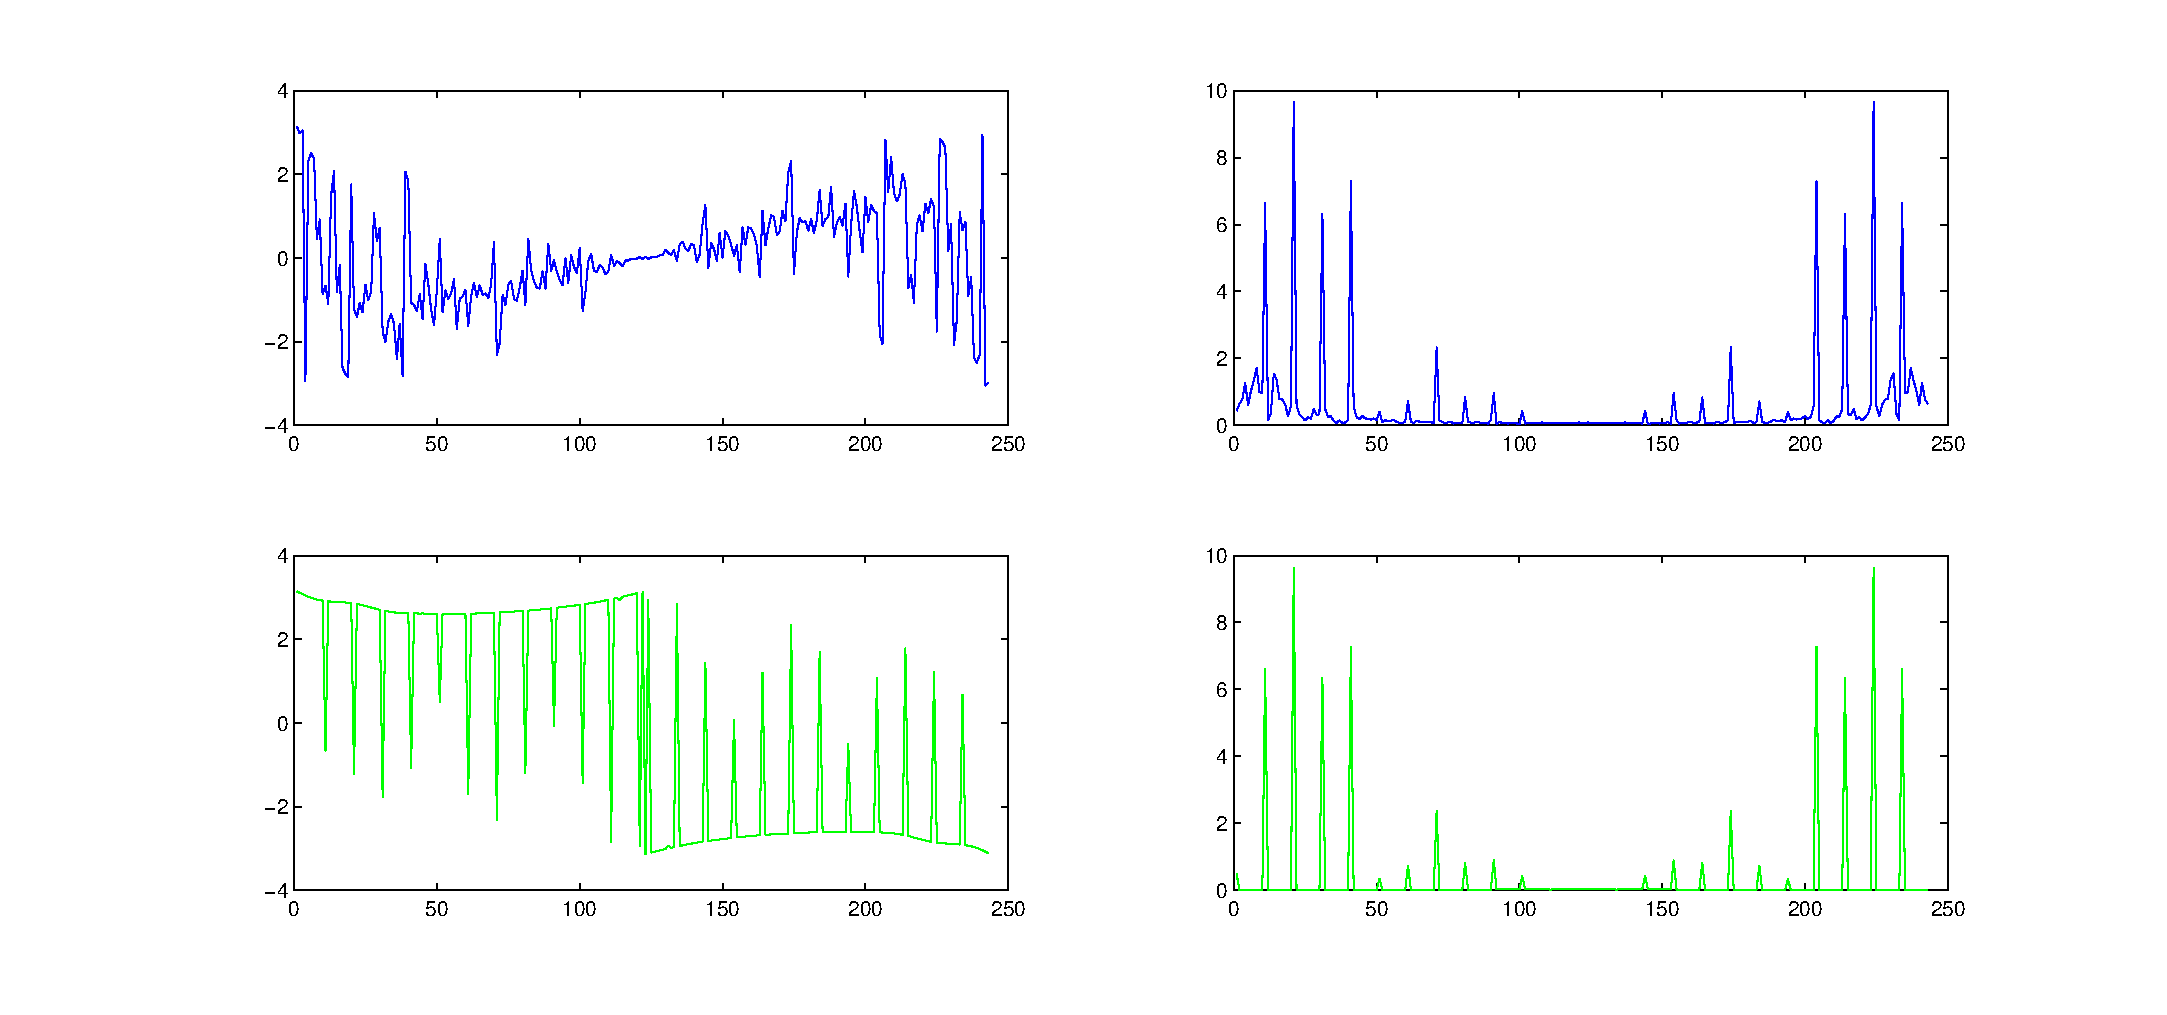
\includegraphics[width=\textwidth]{A1_7.eps}
值得一提的是,一开始我没有对时域信号进行重采样,导致频域滤波的结果幅度特性符合但相位特性偏差很大。重采样以后就可以得到符合要求的特性。这里我选择了10倍,也就是离散基频作为重采样倍数。虽然得到了预期结果,但我仍未完全理解重采样过程起到的作用,如果可能希望老师或助教赐教。
\section{}
\noindent\ding{125}{\CJKfamily{kai}这段音乐的基频是多少?是哪个音调?请用傅里叶级数或者变换的方法分析它的谐波分量分别是什么。提示:简单的方法是近似取出一个周期求傅里叶级数但这样明显不准确,因为你应该已经发现基音周期不是整数(这里不允许使用resample 函数)。复杂些的方法是对整个信号求傅里叶变换(回忆周期性信号的傅里叶变换),但你可能发现无论你如何提高频域的分辨率,也得不到精确的包络(应该近似于冲激函数而不是sinc 函数),可选的方法是增加时域的数据量,即再把时域信号重复若干次,看看这样是否效果好多了?请解释之。}\ding{126}
\par
这段音乐的基频约为329Hz,音名是E。傅立叶变换得到前几个较明显的谐波为[0.6882    1.0000    0.6547    0.7550    0.0413    0.0738    0.2413](已经相对于最强分量归一化)。这里使用的仍是上一节所述的方法,只是按照题目要求没有使用resample,而是使用了时域重复的方法。时域重复搬移对于频域来说相当于采样,可以使谐波分量得到加强,杂波则相对得到削弱。
\section{}
\noindent\ding{125}{\CJKfamily{kai}再次载入fmt.wav ,现在要求你写一段程序,自动分析出这段乐曲的音调和节拍!如果你觉得太难就允许手工标定出每个音调的起止时间,再不行你就把每个音调的数据都单独保存成一个文件,然后让MATLAB 对这些文件进行批处理。注意:不允许逐一地手工分析音调。编辑音乐文件,推荐使用“CoolEdit”编辑软件。}\ding{126}
\par
这一部分是最为花费时间的一部分。首先,要正确地分出乐曲的节拍。一开始我的思路是将时域信号细分,每个小的部分都可以利用上一题的方法求得音调,相同音调属于同一节拍。这一方案最终的效果并不理想,一来音调的判断并不准确,特别是一些部分本身就是两个音调叠加,难以正确分辨。后来我注意到时域信号有幅度的信息,根据前面小题中音符上升、衰减到消失的包络,一种可行的方案是从时域寻找幅度快速上升的分界点,各个分界点之间是同一个音符。后来的实践证明,这一思路相对来说可靠得多。
\par
接下来的工作是确定时域信号包络,基本思路就是低通滤波。滤波器的形状选择我选择了高斯滤波,这在图像处理中大概是最常用的模糊滤镜了。将高斯低通滤波器应用于一维信号,我参考了StackOverFlow上http://stackoverflow.com/questions/6992213/gaussian-filter-on-a-vector-in-matlab的方法,经过参数的调较,得到了较为合理的波形。利用findpeaks函数,较为精确地确定了节拍的分界点。
\par
提取音调信息的功能全部放在了AnalyseTone函数当中。我针对信号的特点进行了一定的预处理,利用与前述相似的方法求出该段音乐的包络,利用包络对信号进行归一化,在一定程度上消除幅度衰减带来的低频分量,提高判断的准确率。提取音调我使用了与前边不同的方法,原因是原有方法准确率太低。由于这里的信号持续时间比较长,混入的噪声比较多、比较杂,难以准确找到正确合理的基频。这里,针对信号为乐音的特点,我针对性地寻找了可能的基频对应各个谐波的总能量,取其最大的对应频率为该段音乐的音调,得到了较为合理的结果。由于有较为复杂的预处理过程,这部分运行稍慢,需要等待几秒钟。最终得到的音调和时长显示在命令行中,figure画出的是时域波形绝对值、包络和分割点,以及柱状图表示的音调和时长。每个柱表示上一个点到该点的音调或时长。时长单位是1/2s,如图所示。
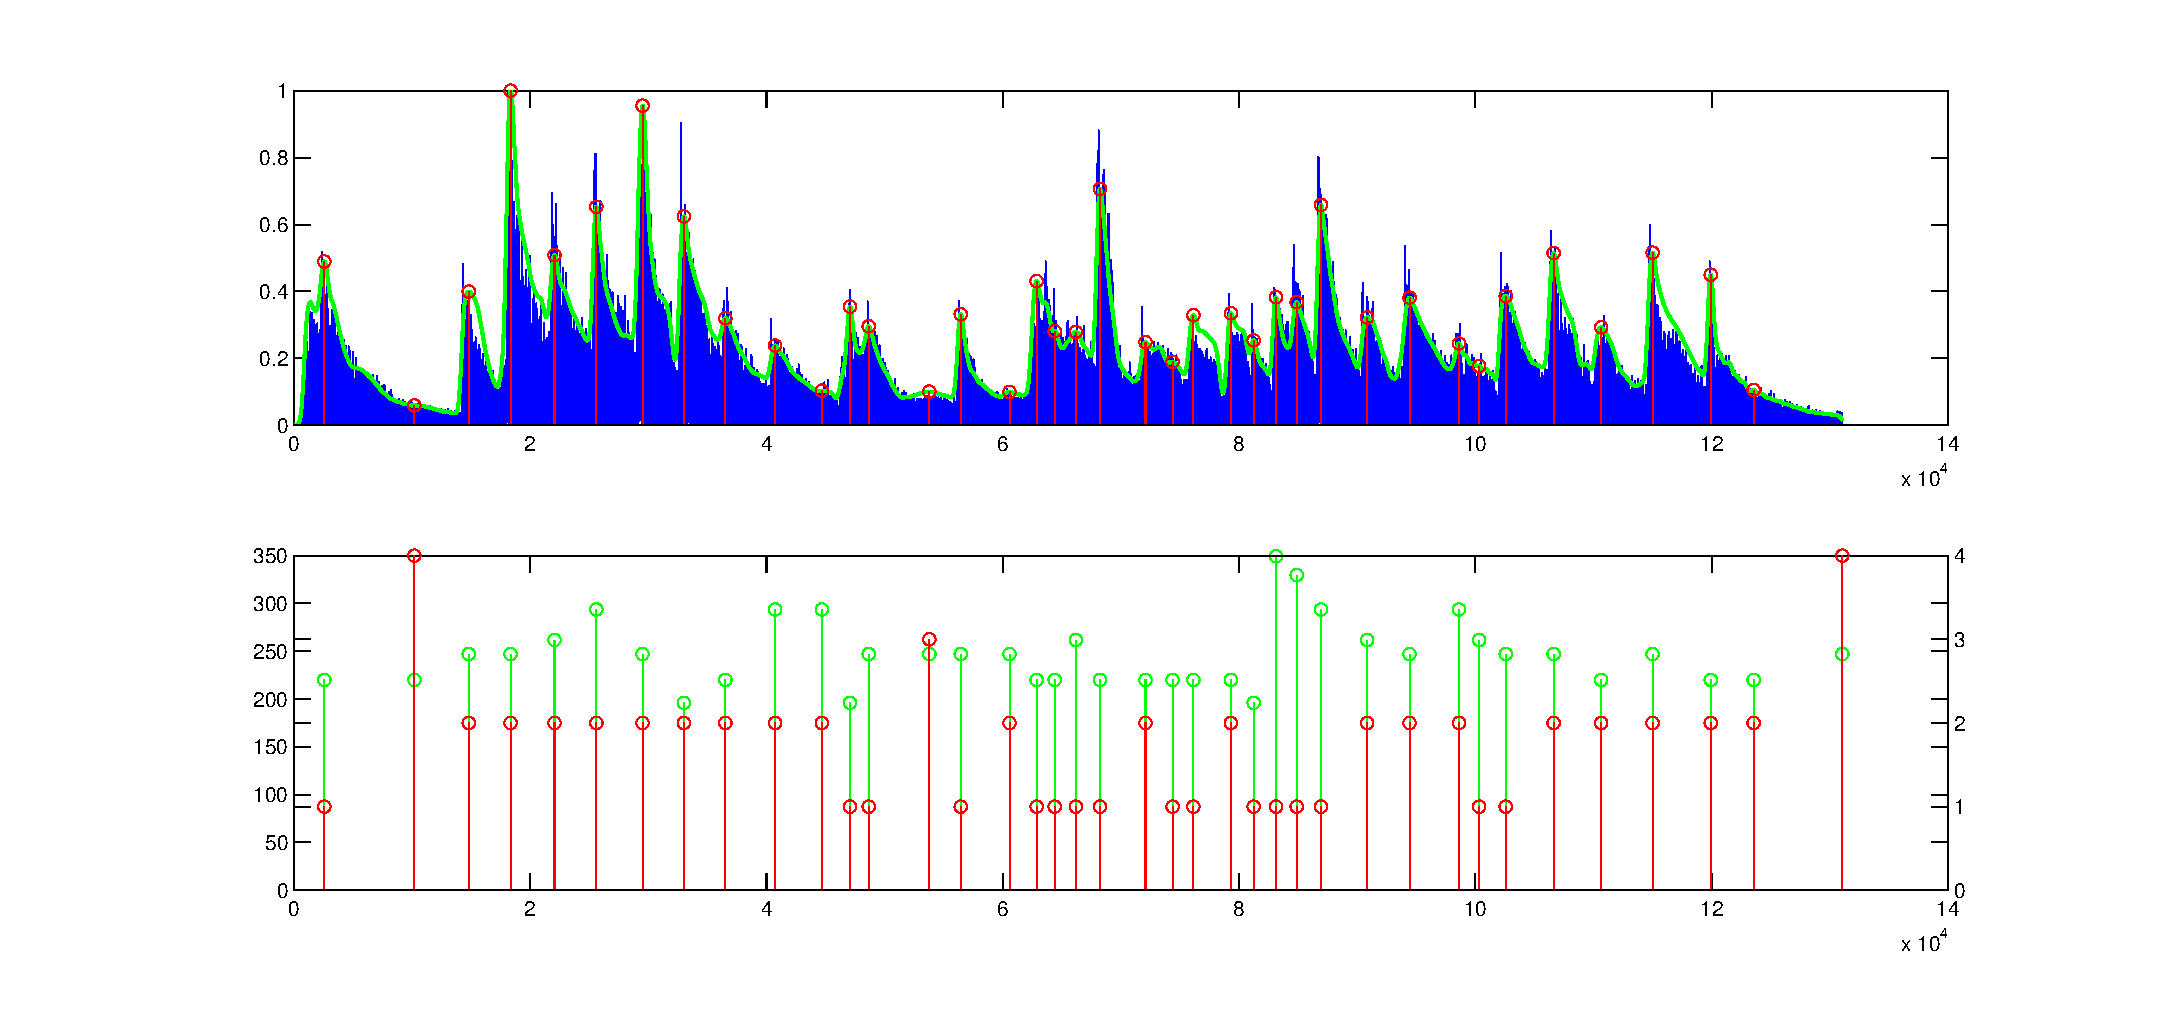
\includegraphics[width=\textwidth]{A1_9.eps}
\par
由于缺乏音乐训练,我无法判断出结果是否完全正确,但整体的大概形状可以确定是合理的。由于findpeaks有一定容差,有一些音符被分开了。
\section{}
\noindent\ding{125}{\CJKfamily{kai}用(7) 计算出来的傅里叶级数再次完成第(4) 题,听一听是否像演奏fmt.wav 的吉他演奏出来的?}\ding{126}
\par
利用GenerateToneLikeGuitar代替GenerateTone。实在话说,不是很像吉他……
\section{}
\noindent\ding{125}{\CJKfamily{kai}也许(10) 还不是很像,因为对于一把泛音丰富的吉他而言,不可能每个音调对应的泛音数量和幅度都相同。但是通过完成第(8) 题,你已经提取出fmt.wav 中的很多音调,或者说,掌握了每个音调对应的傅里叶级数,大致了解了这把吉他的特征。现在就来演奏一曲《东方红》吧。提示:如果还是音调信息不够,那就利用相邻音调的信息近似好了,毕竟可以假设吉他的频响是连续变化的。}\ding{126}
\par
这里由于题给的吉他音域比较低而《东方红》音域较高,即使是邻近音调信息也并不完整,合成的信号仅供示意,我觉得距离真实的吉他差距还是蛮大的。
\section{}
\noindent\ding{125}{\CJKfamily{kai}现在只要你掌握了某乐器足够多的演奏资料,就可以合成出该乐器演奏的任何音乐,在学完本书后面内容之后,试着做一个图形界面把上述功能封装起来。}\ding{126}
\par
这里我没有完全理解题中要求封装的功能具体是什么,我实现的功能是选择调子、乐器、高中低音、唱名和时间,得到单一乐音。调子有C大调和F大调可选,乐器有音叉(无谐波)、风琴(参照题给信息)和吉他(利用前面结果),可选高音、中音、低音共21个音符,时间从0.25s到2s连续可调,波形包络为前面使用过的指数包络。如图所示。
\begin{center}
   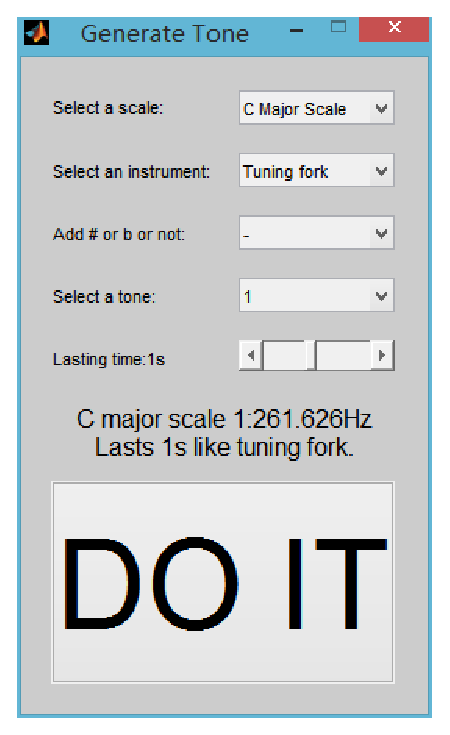
\includegraphics{A1_c.eps}
\end{center}
\XeTeXdefaultencoding GBK
\lstinputlisting{A1_1.m}
\lstinputlisting{A1_2.m}
\lstinputlisting{A1_3.m}
\lstinputlisting{A1_4.m}
\lstinputlisting{A1_5.m}
\lstinputlisting{A1_6.m}
\lstinputlisting{A1_7.m}
\lstinputlisting{A1_8.m}
\lstinputlisting{A1_9.m}
\lstinputlisting{A1_a.m}
\lstinputlisting{A1_b.m}
\lstinputlisting{AddDecay.m}
\lstinputlisting{AnalyseTone.m}
\lstinputlisting{ConcatenateTones.m}
	\lstinputlisting{GenerateTone.m}
\lstinputlisting{GenerateToneLikeGuitar.m}
\lstinputlisting{GenerateToneMoreLikeGuitar.m}
\lstinputlisting{GenerateToneWithHarmonic.m}
\XeTeXdefaultencoding auto
\end{document}